\section{Over all structure}

During the project we have worked on all parts of the system. This section describes the key elements of the overall system when we started the semester, so it is easier to follow the work described throughout the report. 

The GIRAF content is divided into areas of responsibility. This is shown in Figure \ref{fig:ProductStructure}

\begin{figure}[H]
    \begin{center}
        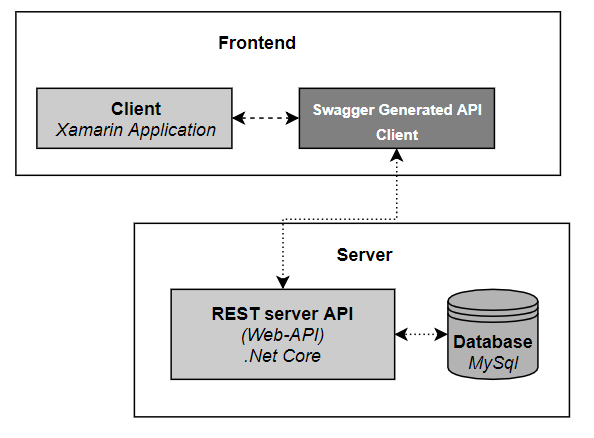
\includegraphics[width=0.95\textwidth]{figures/ProductStructure.png}
    \end{center}
    \caption{Overall structure of the GIRAF content}
    \label{fig:ProductStructure}
\end{figure}

All repositories in the project is stored on the service GitLab, that also provides \gls{ci} for the project. 

\subsection{Frontend}
The Frontend contains the UI elements, called the client, and communication to the server. The client, which contains the UI material for the Weekplanner application uses the Xamarin framework. The framework makes it possible to make both Android and iOS applications. The application is structured with the MVVM pattern, where the models, the view, and the view models are separated. This means that the visual aspects are exclusively placed in the views, the business logic in the view models and the data objects that represent the data from the database in the models.

The communication between the client and the Web-API are done through an API client. In this report this is called the \gls{fapi}. The \gls{fapi} are auto generated by the software Swagger.

\subsection{Server}
The server contains both the database and the Web-api. The Web-api exposes endpoints to the \gls{fapi} and communicates with the database. It is build with the Rest principles. This means that it must uphold the following six guidelines\cite{REST}. 
\begin{itemize}
    \item Separate user interface and server. This makes it easier scale and to move the UI to a different platform.
    \item The server should be stateless, so all the needed information should be stored in a request rather than as context on the server.
    \item Response data should be cacheable, so a client has the right to store and reuse response data for later requests. 
    \item Software engineering principles of generality should be applied to component interface. This means upholding four interface constraints: identification of resources, manipulation through constraints, self-descriptive messages and hypermedia as the engine of application state. 
    \item The system should be hierarchically layered, and a component should not be able see or interact behind the immediate layer.
    \item A client should be able to extended functionality with applets or scripts. This is optional
\end{itemize}

The database is a MySQL database. It is build with the structure shown in \ref{fig:state-at-handoff:db}

\begin{figure}[ht]
    \centering
    \caption{Diagram of \gls{er} diagram at the time of handoff}
    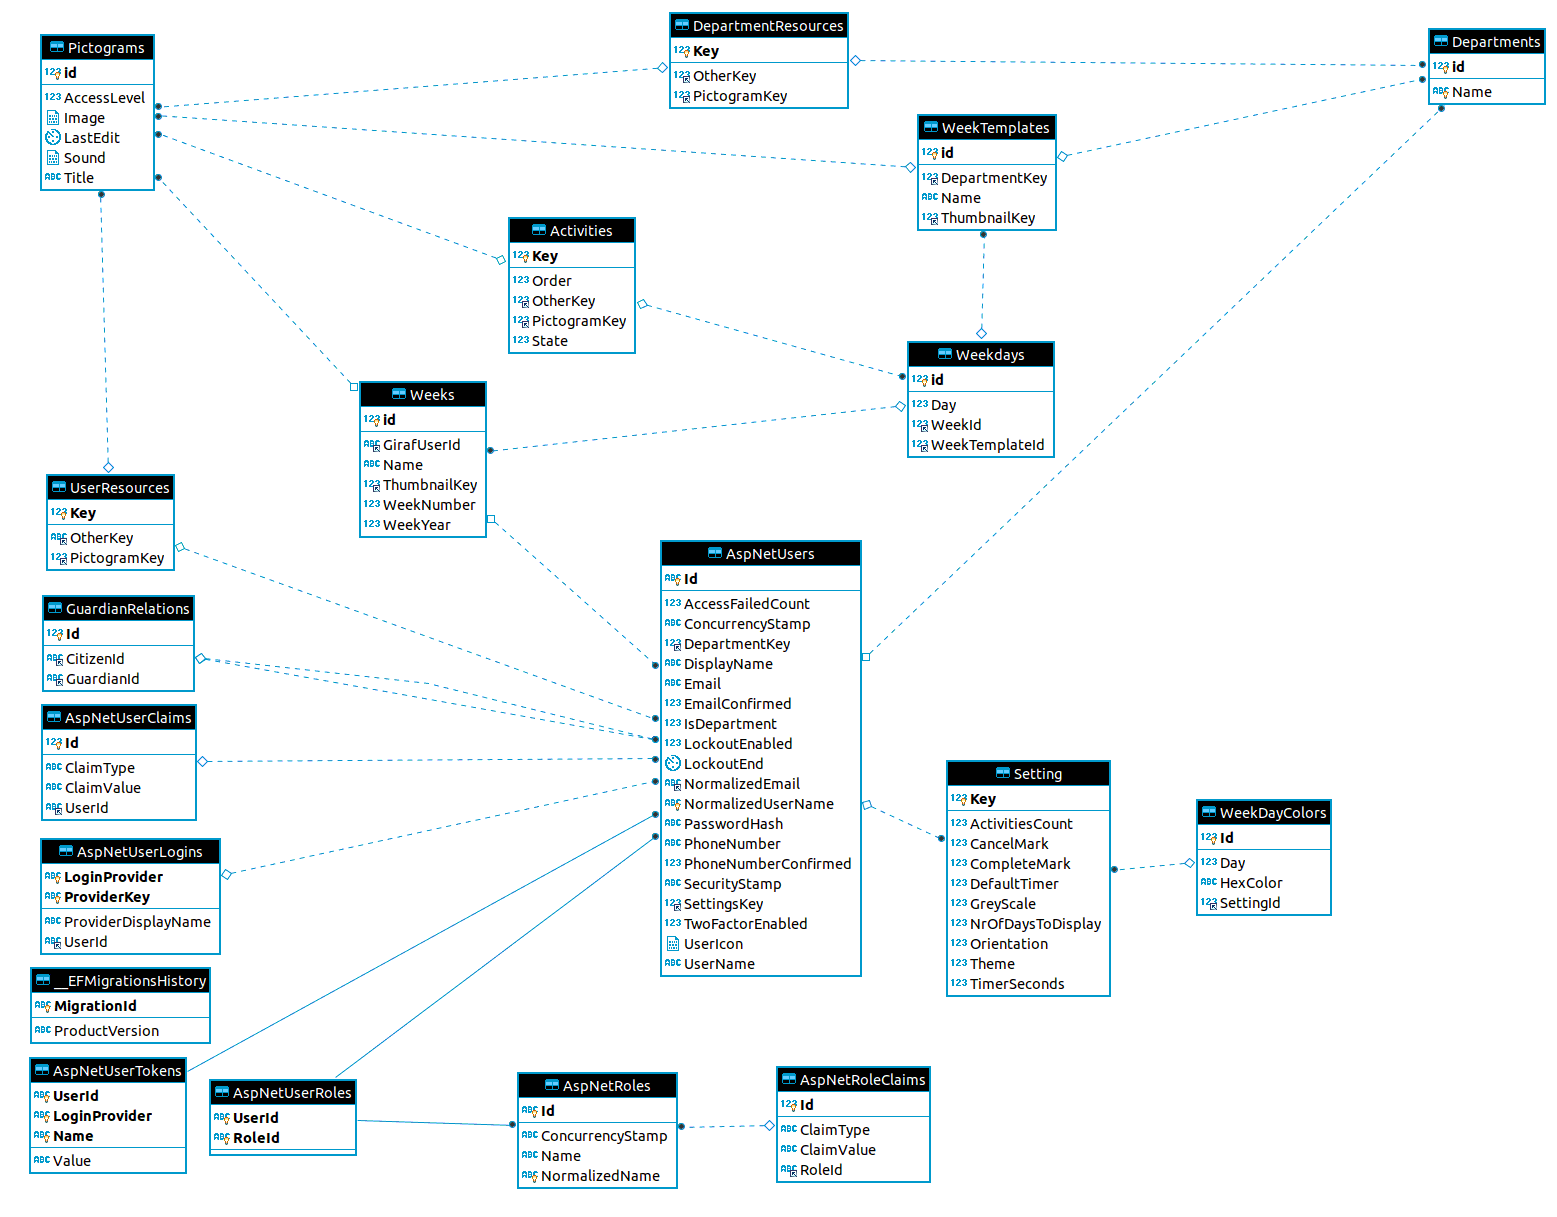
\includegraphics[width=1\textwidth]{figures/db_ho.png}
    \label{fig:state-at-handoff:db}
\end{figure}

\todo{Hvad er de stiblede linjer}

All the server content is hosted in Docker, a operating-system level virtualization. The content is divided into containers whenever possible. 

Some of the containers are set up in clusters, using the Kubernetes managing system. The rest of the containers are planned to be migrated, but have not been moved yet. \ref{fig:state-at-handoff:server} complete overview of the servers and which services they run.

\begin{figure}[h]
    \centering
    \caption{Diagram of the server setup at the time of handoff\cite[p.~74]{SW611F18}}
    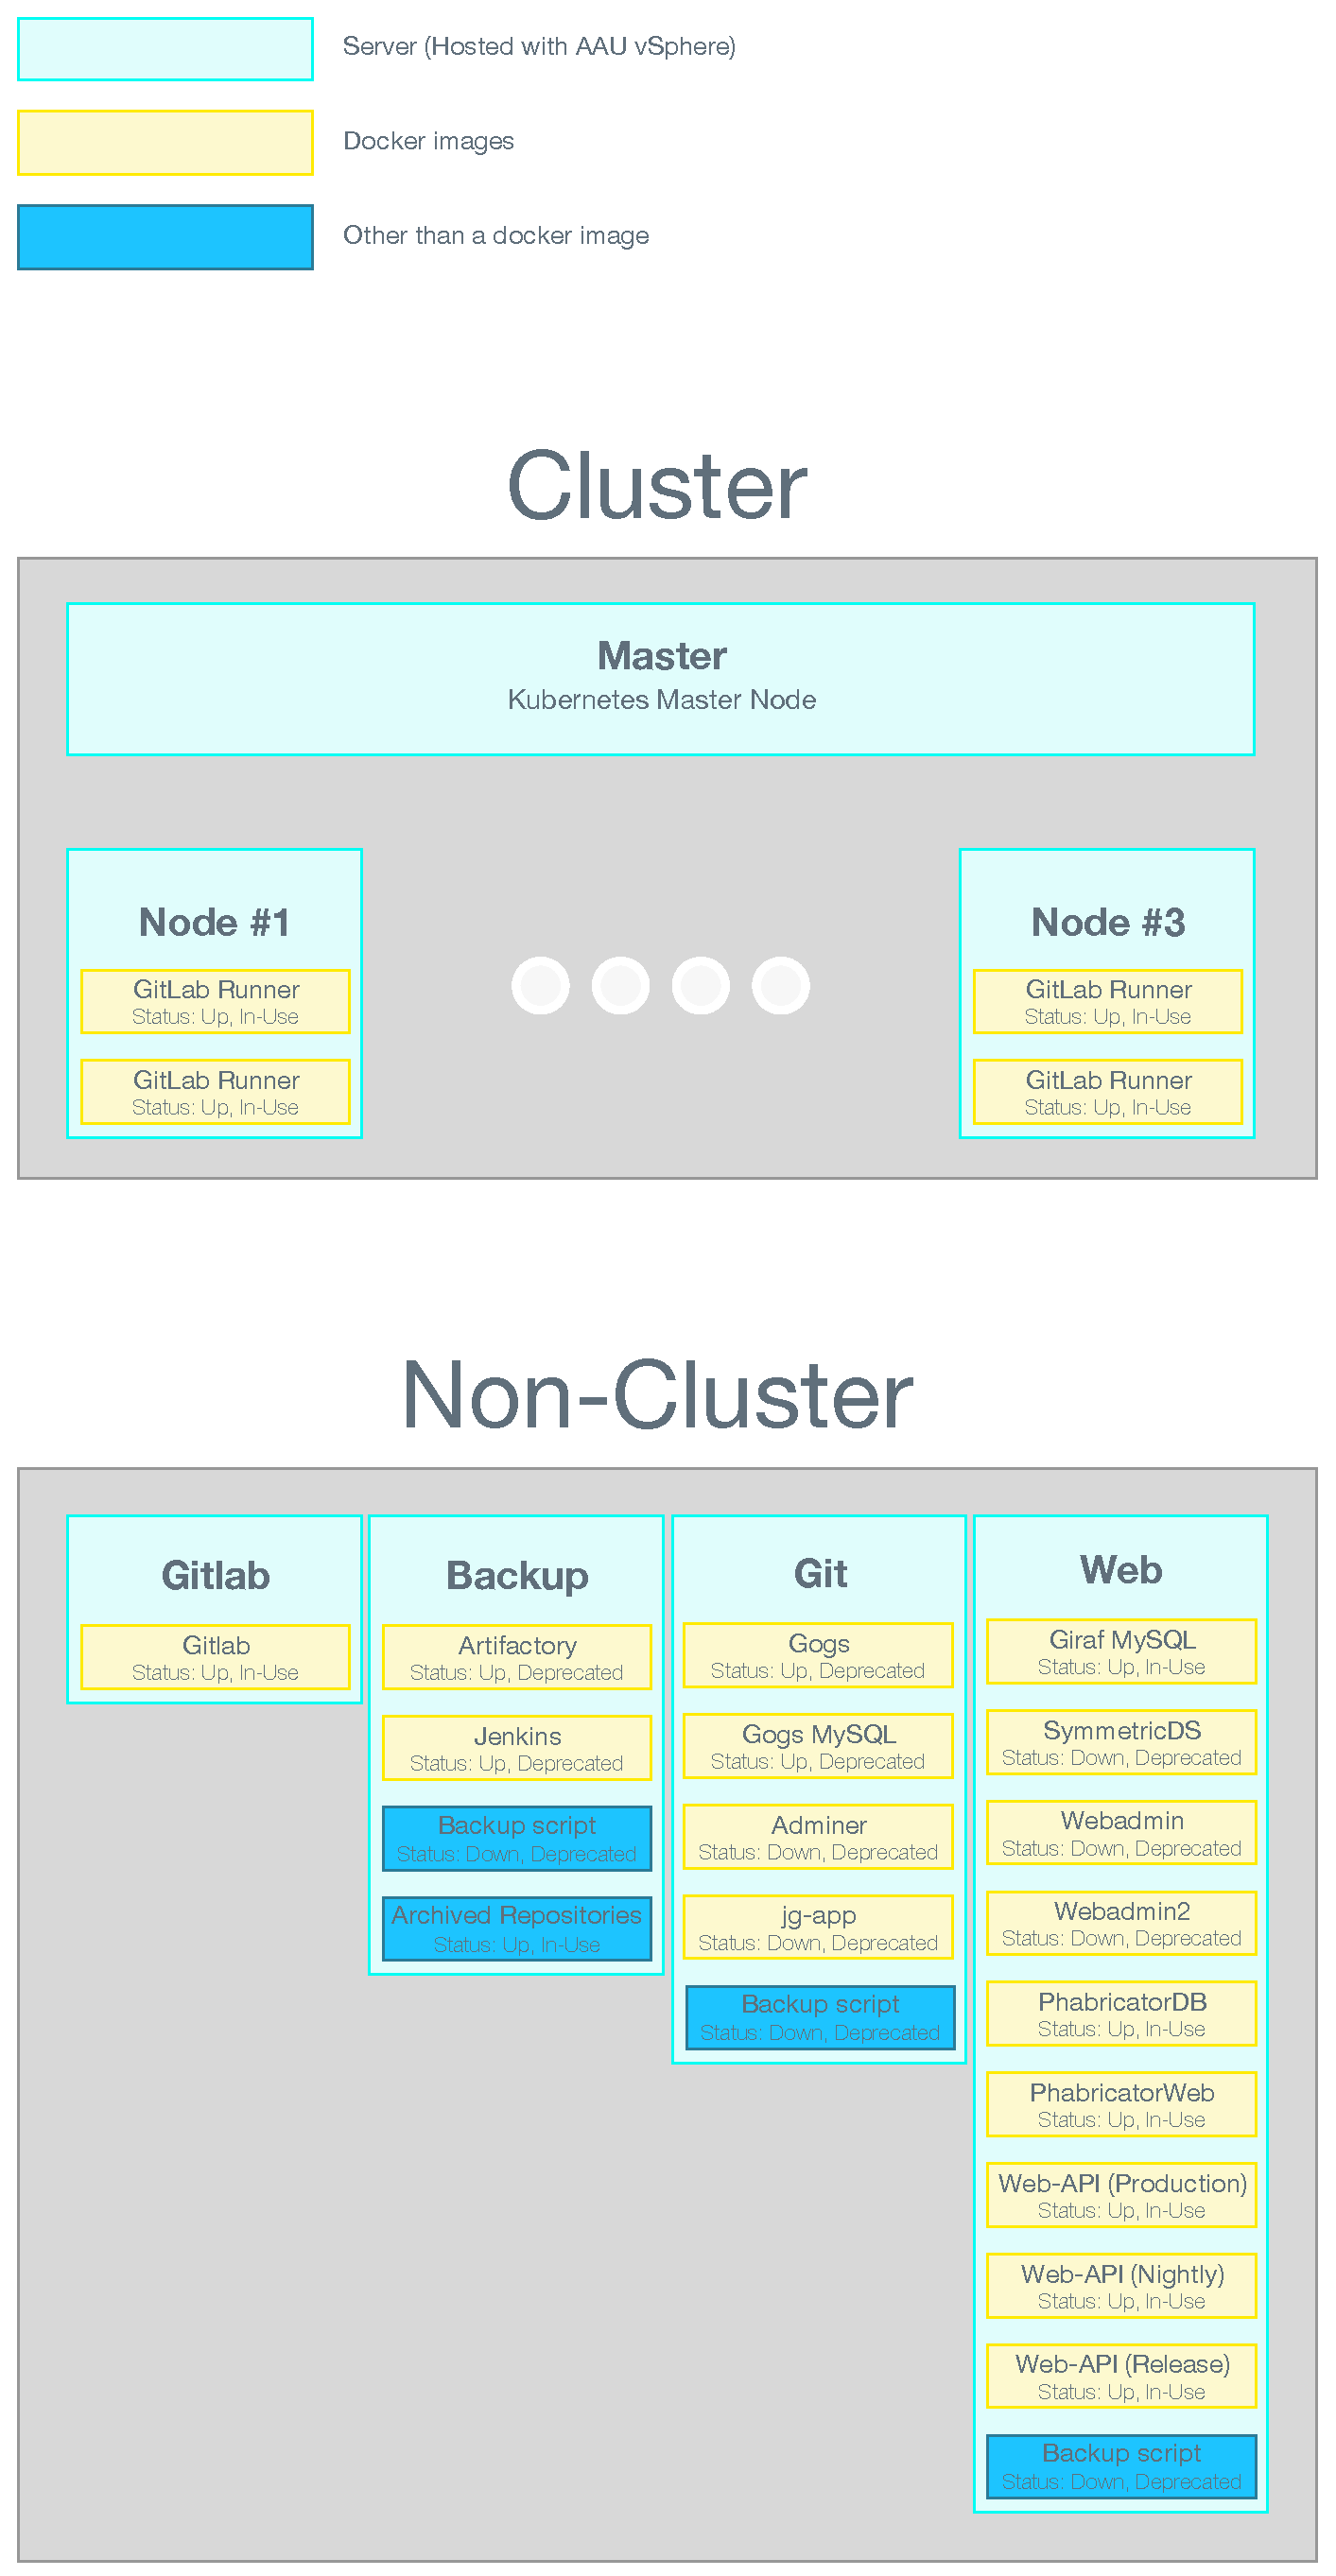
\includegraphics[height=1\textheight]{figures/Server-Overview.pdf}
    \label{fig:state-at-handoff:server}
\end{figure}

This shows that it is only the GitLab Runner nodes that have been moved to Kubernetes. 




